\chapter{Methodology} \label{CH:method}
%This section will focus on the story of how the current model came to be. \\
%Start with the beginning: look on Box for presentations\\
%TIMELINE:\\
%
%
%Feb 2018 - PLIC reconstruction- area of discontinuity $\rightarrow$ velocity to drive back discontinuity\\
%Apr 2018 - velocity correction based on area times some factor $\rightarrow$ gives idea fro subgrid HFM\\
%May 2018- using matlab compute heights and curvature as 1/r \\
%Jun 2018 - Can show 5th order L2 error with mesh refinement (5th order finite difference scheme)\\
%Jul 2018 - ICLASS 2018 Poster - here we've tried several different discretization techniques\\
%Aug 2018 - Reintroduce SG velocity but allow to be influence by curvature rather than area\\
%Oct 2018 - Implement FG HFM but find parasitic wiggles $\rightarrow$ this is start of Herrmann correction and we add in 2nd pressure equation to ensure fine grid divergence free condition (12Oct18 presentation - late october is basically final APS presentation... same with november... thats the state at that point in time )\\
%Jan 2019 - Found discrepancy in Herrmann Eqn \\
%Mar 2019 - delta approximation big parametric study \\
%Apr 2019 - still doing para study \\

%Method development which would include information from the fine grid to reduce interface reconstruction discontinuities. 
%
%Introducing a fine grid velocity 

%With the standard implementation of NGA, VOF is calculated on the fine grid and curvature is computed on the coarse grid. 
%
%
%
%\begin{figure}[htbp]
%	\centering
%	\begin{tikzpicture}[scale=1.5]
%	% PLIC
%	\draw [lightblue,fill=lightblue] (0,0) -- (0,0.7) -- (1,0.7) -- (1,1.3) -- (2,1.3) -- (2,0) -- cycle;	
%	% VOF
%	\node at (0.5,0.5) {0.7};
%	\node at (1.5,0.5) {1};
%	\node at (0.5,1.5) {0};
%	\node at (1.5,1.5) {0.3};
%	%Cell
%	\draw [black, very thick] (0,0) -- (2,0) -- (2,2) -- (0,2) -- (0,0);
%	% Grid
%	\draw [blue, thick, dashed] (1,0) -- (1,2);
%	\draw [blue, thick, dashed] (0,1) -- (2,1);
%	\draw [arrows=->,line width=1.0] (0.5,0.7) -- (0.5,1.3);\node [left] at (0.49,1.1) {\scriptsize $v$};
%	\draw [arrows=->,line width=1.0] (1.7,1.7) -- (1.7,1.3);\node [right] at (1.705,1.5) {\scriptsize $v$};
%	\end{tikzpicture}
%	\caption{Advection of a one-dimensional fluid interface}
%	\label{fig:1Dadvect}
%\end{figure}

%\subsection{Oscillating Droplet Test Case}
%To further quantify the problem that is occurring, a baseline test case which highlights the shortcomings of current methods is necessary. To this end, an oscillating two-dimensional droplet is used to assess the height function method and the proposed solution methods. This test case was chosen as it is considered a standard benchmark problem for testing the accurate prediction of multiphase flow behavior\cite{Salih2002}. Additionally, for the height function method, the oscillating droplet offers an extensive testing of interface orientations which is important for measuring the robustness of the method. The interface is initialized with an ellipsoid. Surface tension drives the droplet's semi-major axis to fluctuate between alignment with the $x$ and $y$ axes. The period of oscillation $T_{e}$, is a function of surface tension coefficient ($\sigma$), density ($\rho_l$ and $\rho_g$), and equivalent circular radius($R$), and can be computed analytically as~\cite{Rayleigh}
%\begin{equation}
%T_{e} = 2 \pi \sqrt{\frac{(\rho_{l}+\rho_{g})R^3}{6\sigma}}.
%\label{period}
%\end{equation}
%
%To establish successful algorithm performance of NGA, an alternate curvature scheme was selected and an oscillating droplet test case ran. Simulation parameters include a density ratio of 1000, viscosity in both the liquid and gas phases are 0, and no walls are present in the computational domain. For the initial baseline, a mesh of 64x64 grid cells make up the domain. A semi-major radius of 0.24 and a semi-minor axes radius of 0.20 define the initial displacement of the droplet. The total domain length is set to 1.0. These parameters are chosen as they align with the analytic solution assumptions made. Figure \ref{fig:acesKE} shows kinetic energy conservation through the progression of the simulation. Simulation success is quantified by normal periods of oscillation and diminishing kinetic energy with time. Close adherence to this model can be used as a measure of success with cases from here forward and this case will be plotted with all further test cases. 
%
%\begin{figure}[h]
%	\centering
%	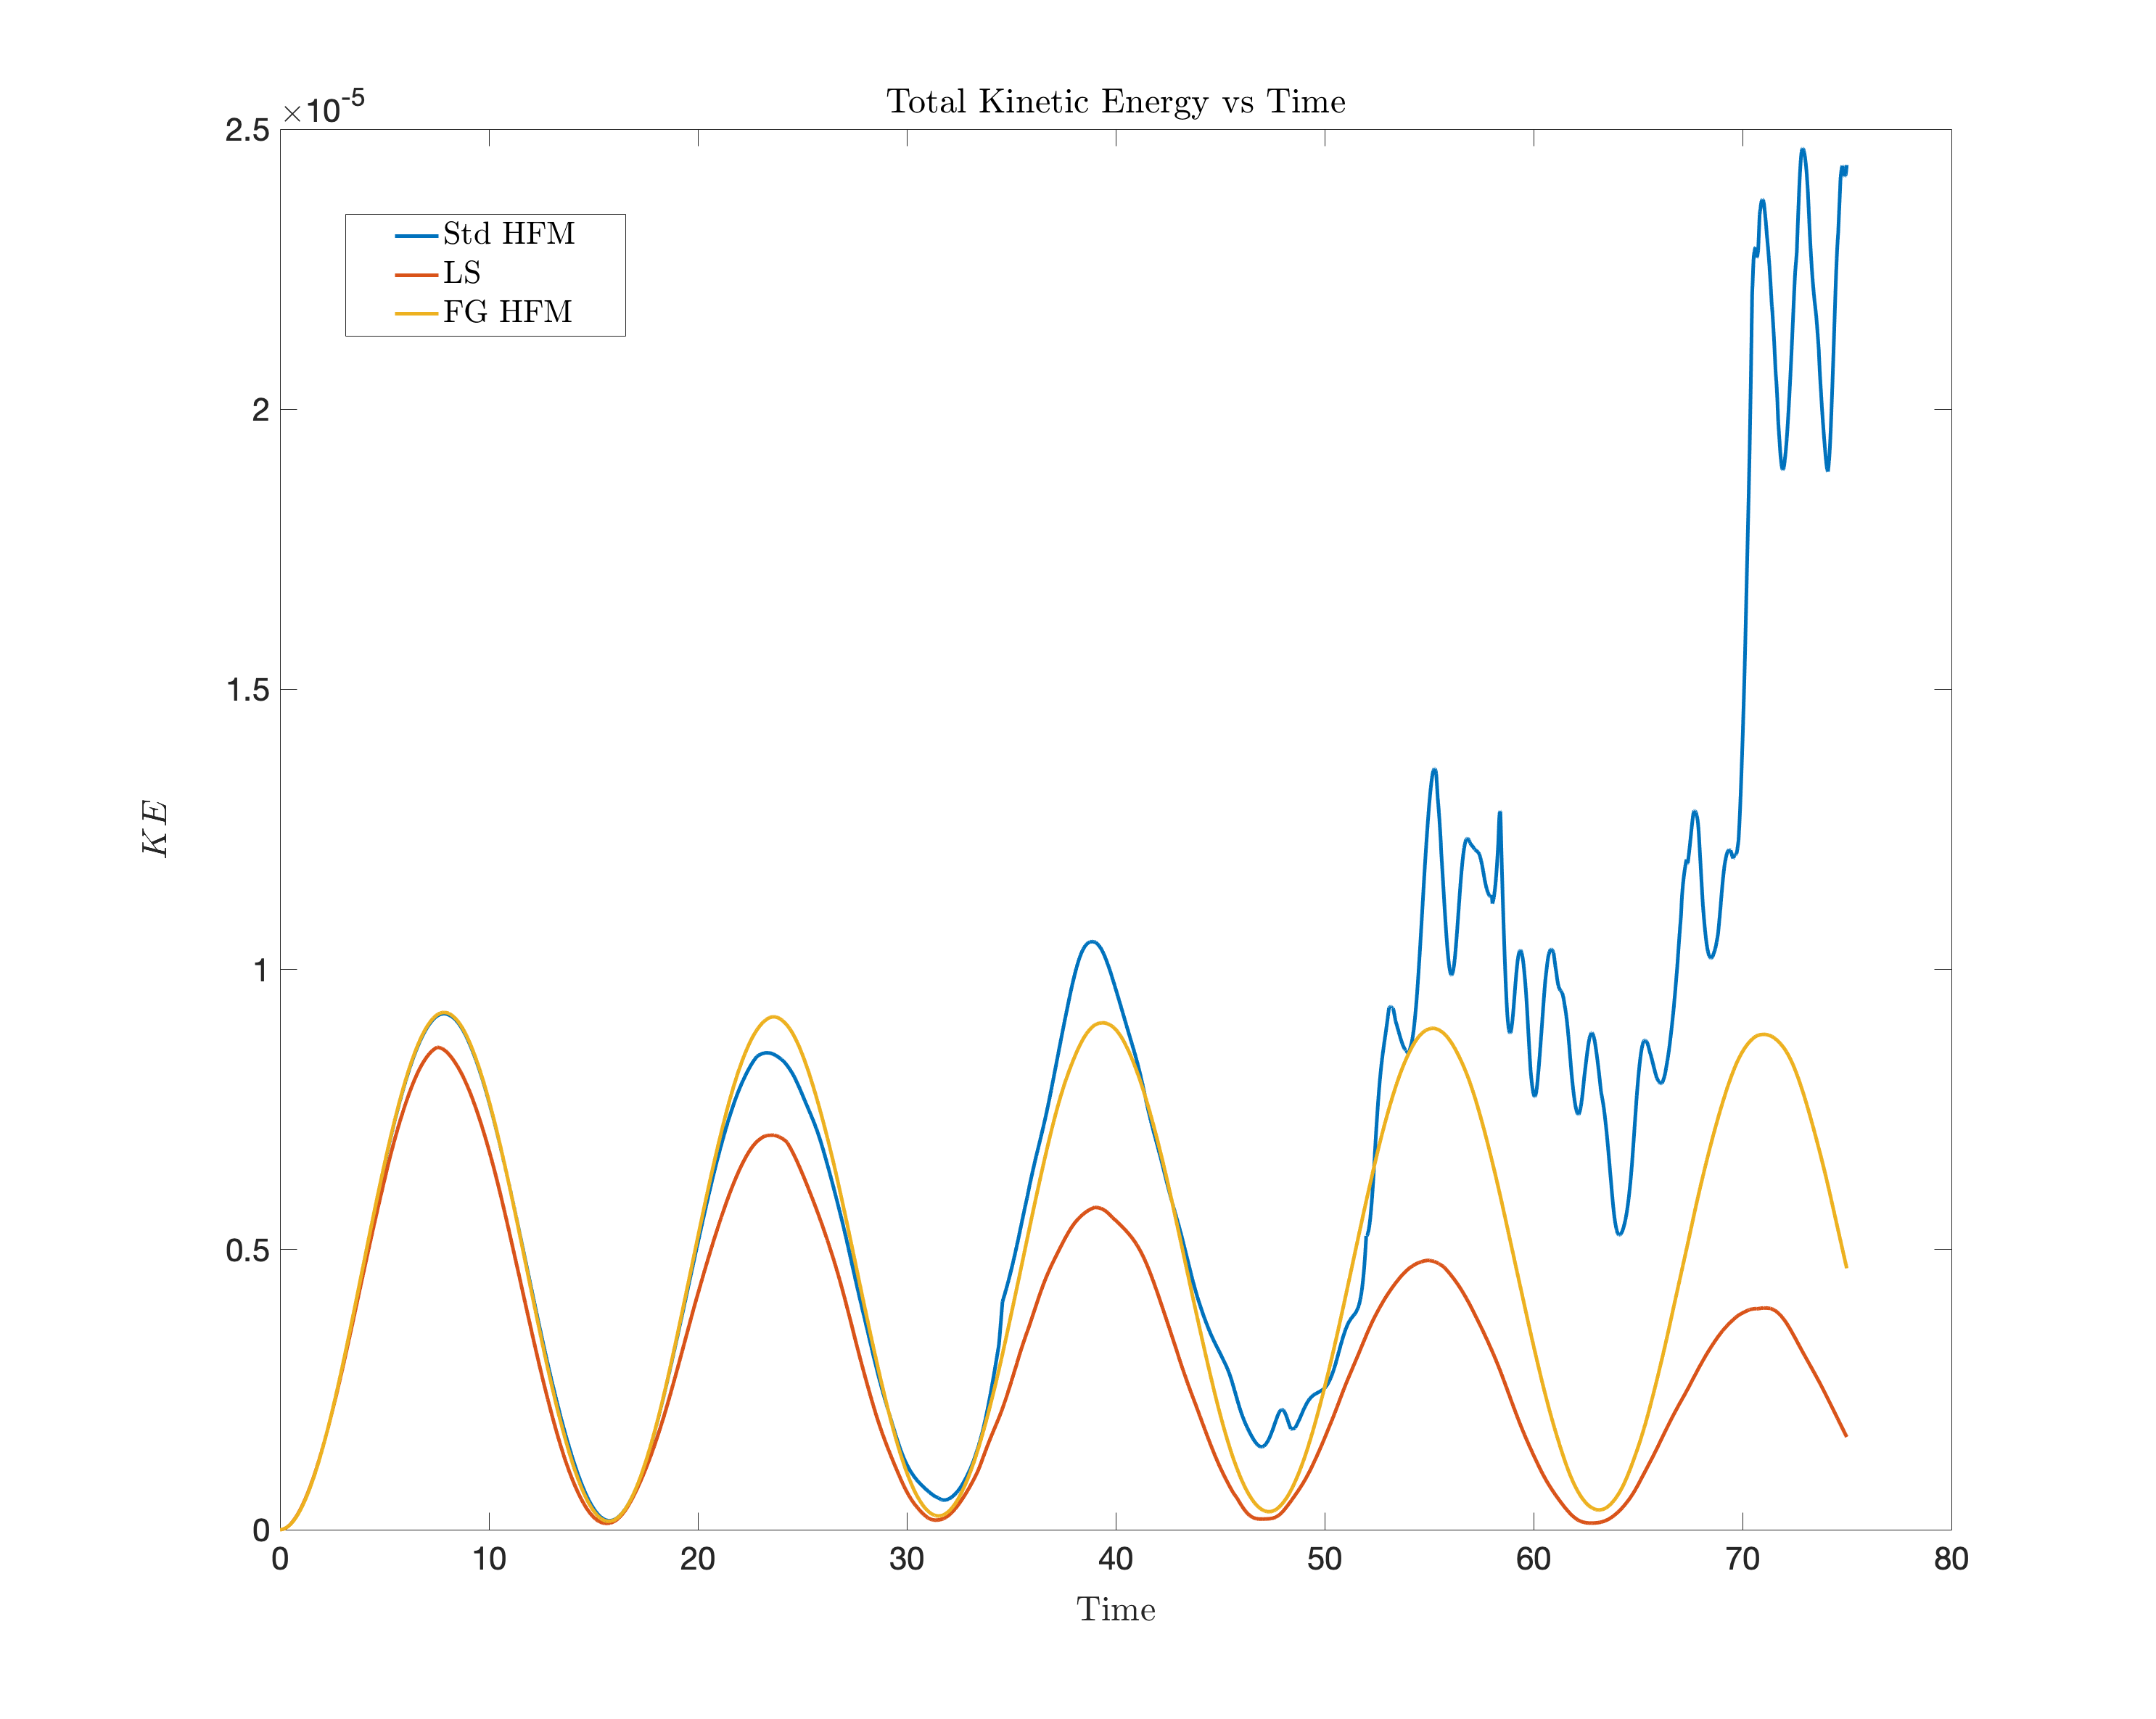
\includegraphics[width=5.0in]{figs/KEvT}
%	\caption{Kinetic Energy with Time \hl{THIS IS NOT THE CORRECT FIGURE}}
%	\label{fig:acesKE}
%\end{figure}
%
% Alternatively, Figure \ref{fig:stdKE} shows the result of the same test case ran with a standard, coarse grid, curvature estimation scheme. The uncontrolled growth seen in the kinetic energy of the standard method is a result of the aformentioned interfacial perturbations. The curvature estimation error and resulting non-physical dynamics are the basis for this research. 

%\begin{figure}[h]
%	\centering
%	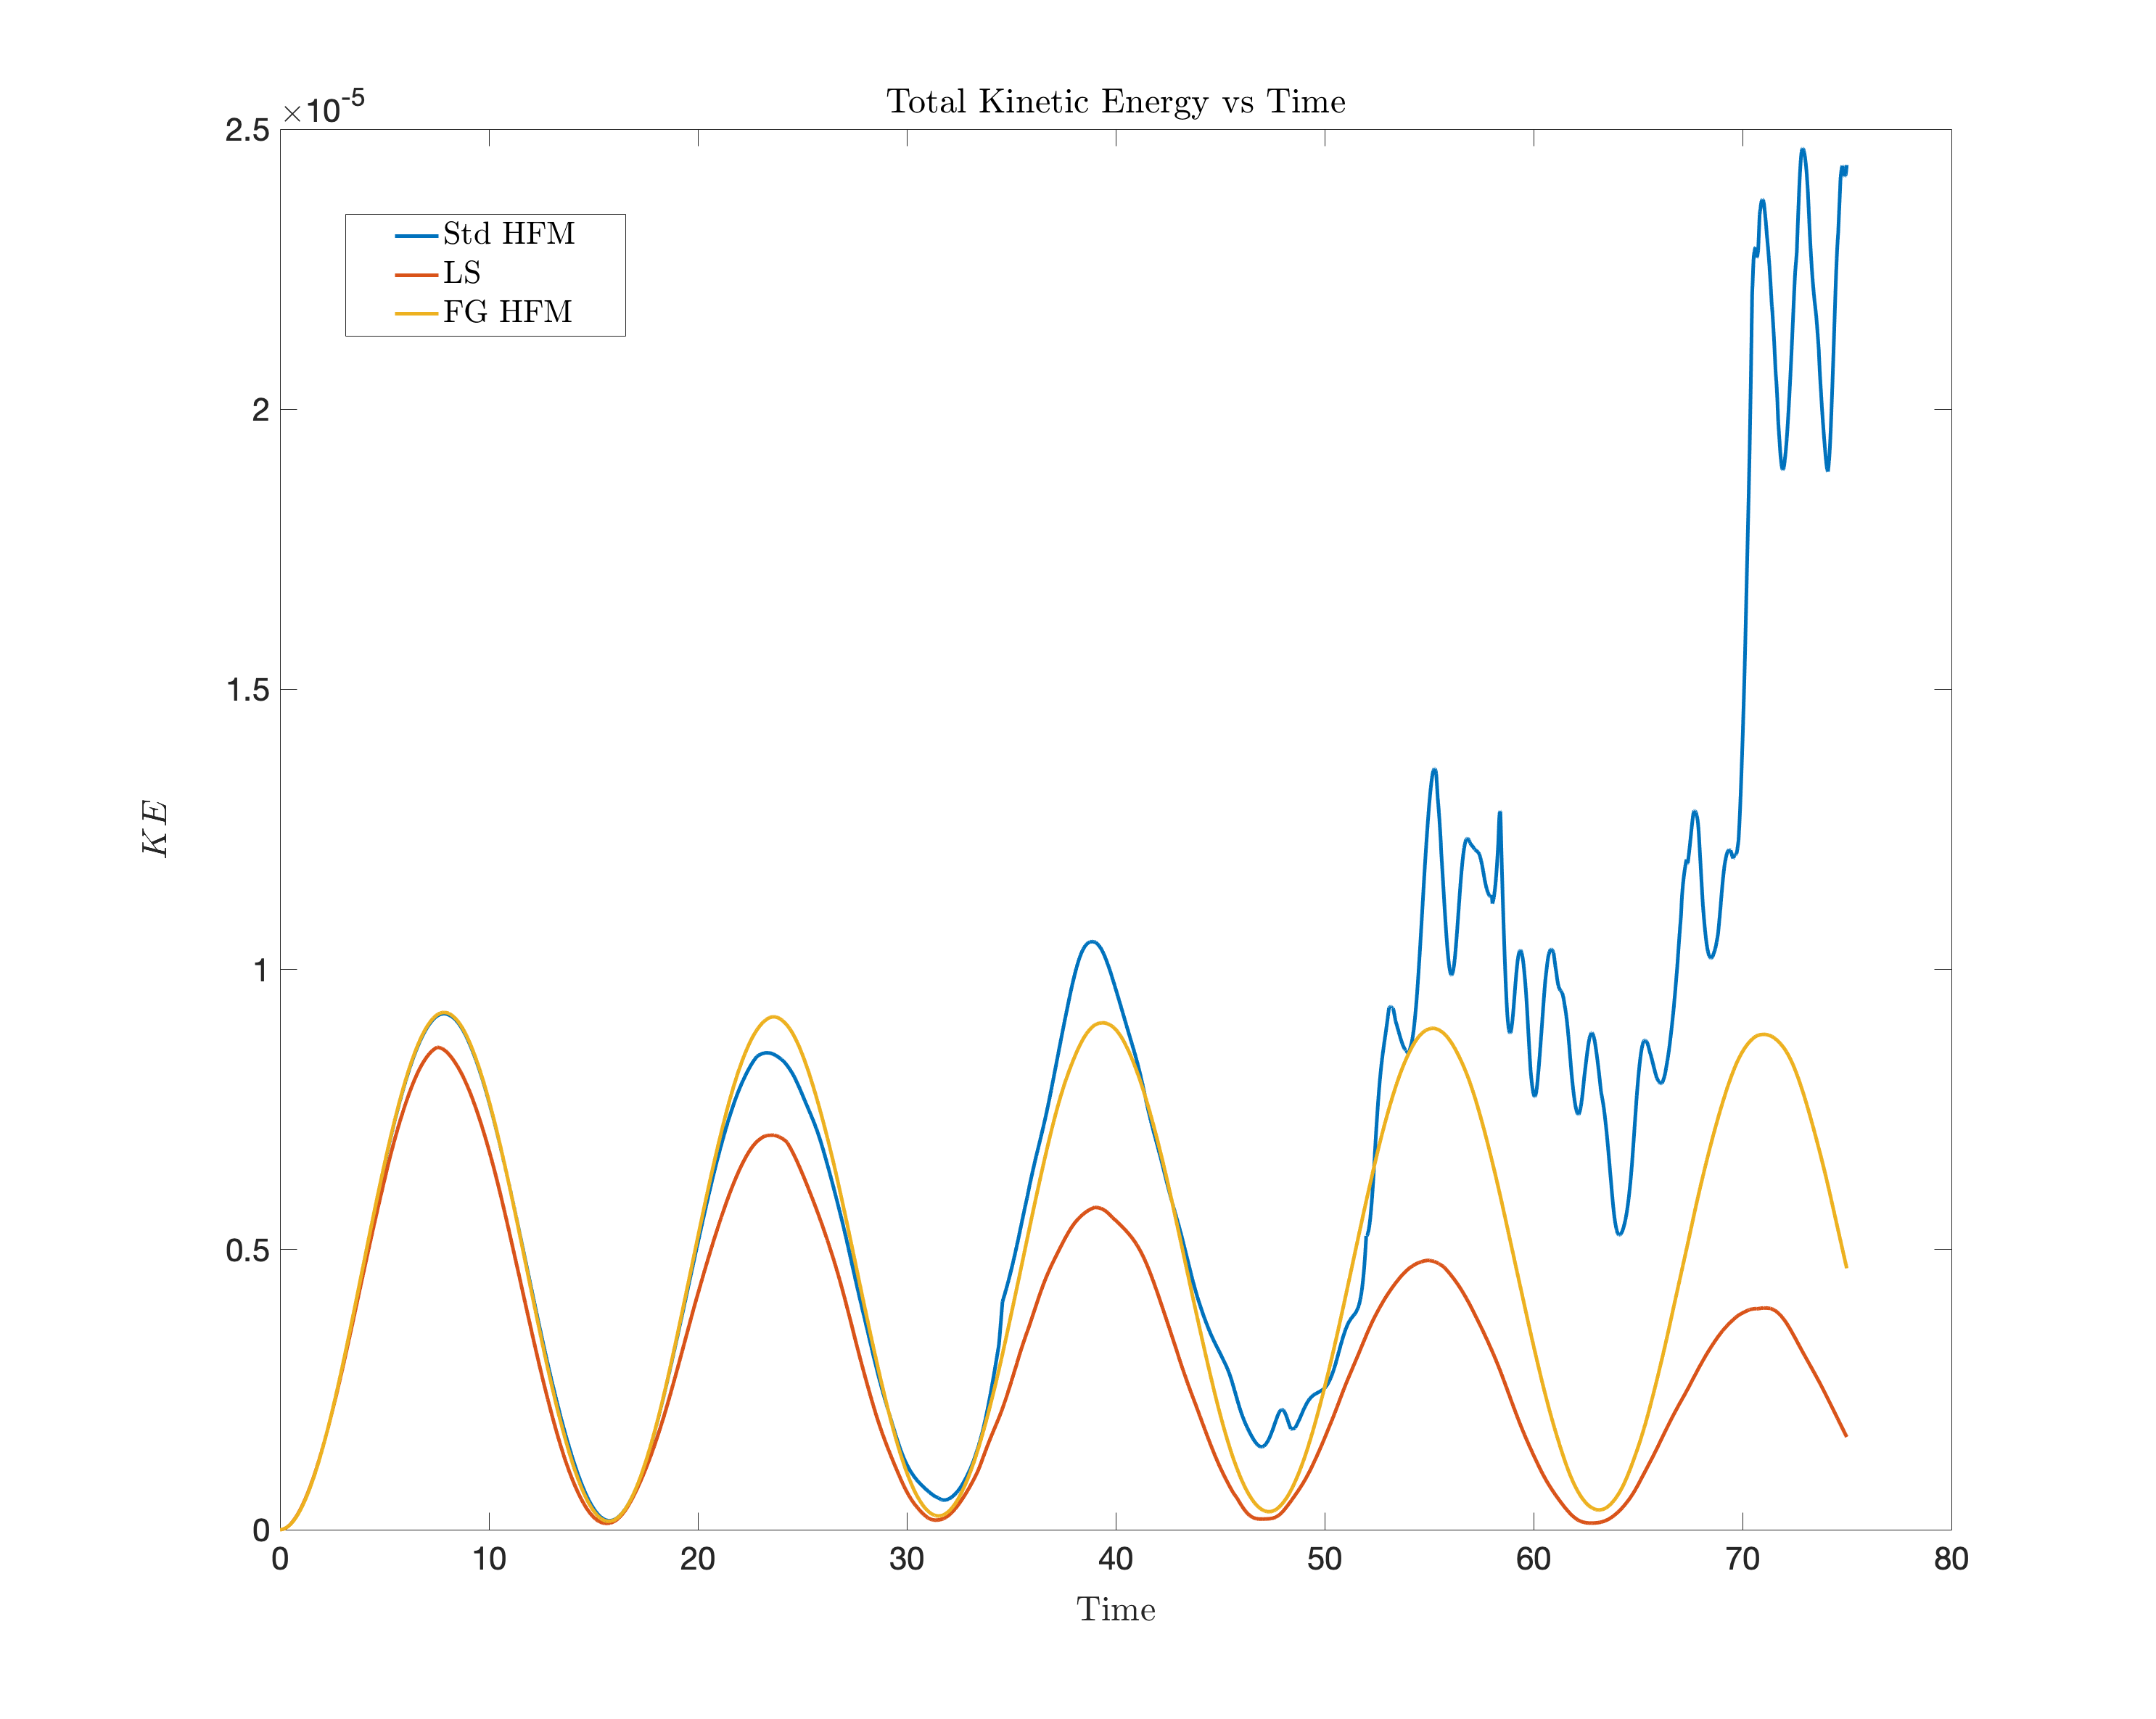
\includegraphics[width=5.0in]{figs/KEvT}
%	\caption{Kinetic Energy with Time \hl{THIS IS NOT THE CORRECT FIGURE}}
%	\label{fig:stdKE}
%\end{figure}

The aim of this research is to allow the coarse grid to be aware of information from the fine grid. The following section will describe several methods which have been proposed and discuss the strengths and shortcomings of each.

When considering how to inform the coarse grid from the finer mesh, a natural direction is to adopt a height function method directly onto the fine grid. Implementing a height function is straightforward as previously described and, the same curvature stencil should result in a more accurate curvature estimation as there is more information available. Figure \ref{fig:fgHFM} gives an example of what this could look like. 
\begin{figure}[h]
	\centering
	\begin{tikzpicture}[scale=1.5]
	% Liquid
	\draw [line width=0,fill=lightblue] (0.5,3.5) to[out=20,in=170] (4,4.5) to[out=-10,in=100] (7.0,0.5);
	\draw [lightblue,fill=lightblue] (0.5,3.5) -- (7.0,0.5) -- (0.5,0.5) -- cycle;
	% \node [] at (0.25,3.5) {$\Gamma$};
	% Mesh
	\draw [step=1.0, help lines] (0.5 , 0.5) grid (7.5,5.5);
	\draw [dashed,step=0.5, help lines] (0.5 ,0.5) grid (7.5,5.5);
	% kappa 1
	\draw [fill] (3.5,4.55) circle [radius=0.1];
	\node [above right] at (3.5,4.55) {$\kappa$};
	\draw [arrows=->,line width=1.0] (2.25,2) -- (2.25,4.3);\node [below] at (2.15,2.15) {\scriptsize $h_{\text{-}3}$};
	\draw [arrows=->,line width=1.0] (2.75,2) -- (2.75,4.45);\node [below] at (2.70,2.15) {\scriptsize $h_{\text{-}2}$};
	\draw [arrows=->,line width=1.0] (3.25,2) -- (3.25,4.53);\node [below] at (3.25,2.15) {\scriptsize $h_{\text{-}1}$};
	\draw [arrows=->,line width=1.0] (3.75,2) -- (3.75,4.54);\node [below] at (3.75,2.15) {\scriptsize $h_{1}$};
	\draw [arrows=->,line width=1.0] (4.25,2) -- (4.25,4.44);\node [below] at (4.25,2.15) {\scriptsize $h_{2}$};
	\draw [arrows=->,line width=1.0] (4.75,2) -- (4.75,4.27);\node [below] at (4.75,2.15) {\scriptsize $h_{3}$};	    
	\end{tikzpicture}
	\caption{Fine grid height function}
	\label{fig:fgHFM}
\end{figure}
 
 
 \subsection{Fifth Order Height Function Method}

\begin{figure}[htbp]
	\centering
	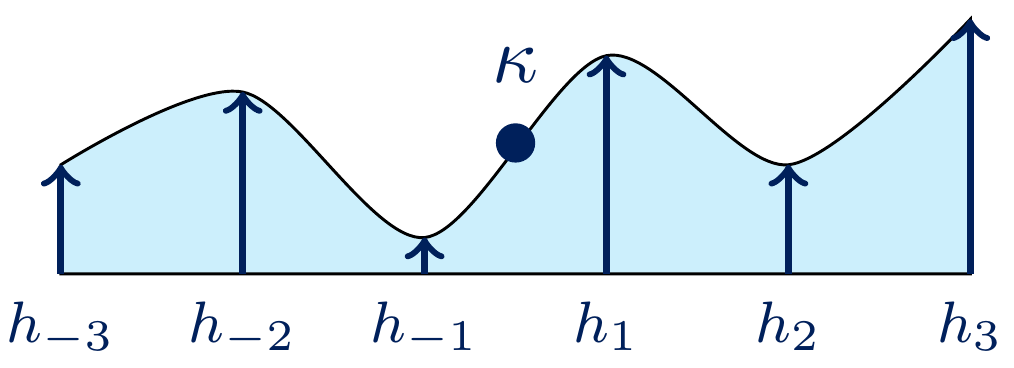
\includegraphics[width=0.5\textwidth]{figs/5thorder.png}
	\caption{$5^{th}$ order scheme.}
	\label{fig:5th} 
\end{figure} 

As seen in Figure \ref{fig:fgHFM}, there are now six columns over which information is being provided. With this information, it is possible to derive fifth order approximations for the first and second derivatives needed for the curvature calculation. Figure~\ref{fig:5th} gives an approximate representation of what a fit might look like for a given point. A general formula for deriving a finite difference approximation given a set of points is given by equations~\ref{eqn:gen}  \& \ref{eqn:poly}. 
\begin{equation}
f'_j + \sum_{k=0}^{2} a_k f_{j+k} = O(?)
\label{eqn:gen}
\end{equation}
\begin{equation}
\frac{dh}{dx} = a_{-3}h_{-3} +a_{-2}h_{-2} + a_{-1}h_{-1} + a_{+1}h_{+1} + a_{+2}h_{+2} + a_{+3}h_{+3} 
\label{eqn:poly}
\end{equation}
\noindent Here, $a_k$ are the coefficients associated with the linear Taylor series which need to be solved for~\cite{moin}. For the six heights given by our fine grid stencil Table \ref{tab:findiff} shows how the linear equations can be formed to find the first derivative.


\begin{table}[htbp]
	\centering
	\caption{Taylor Series Table}
		\begin{tabular}{c|c|c|c|c|c|c|c} % <-- Alignments: 1st column left, 2nd middle and 3rd right, with vertical lines in between
			\textbf{}          &\textbf{$f$} & \textbf{$f'$}            & \textbf{$f''$}                                 & \textbf{$f'''$}                                 & \textbf{$f^{iv}$}                             & \textbf{$f^{v}$}                                \\
			\hline
			$f'$                                     & 0                                     & 1                                                       &                                                    0       &                                                              0&                                                      0&                                                                     0&\\
			$a_{\text{-}3}f_{\text{-}3}$& $\frac{a_{\text{-}3}}{0!}$ &$a_{\text{-}3}\frac{(\text{-}3h)}{1!}$ &$a_{\text{-}3}\frac{(\text{-}3h)^2}{2!}$  &$a_{\text{-}3}\frac{(\text{-}3h)^3}{3!}$   &$a_{\text{-}3}\frac{(\text{-}3h)^4}{4!}$    &$a_{\text{-}3}\frac{(\text{-}3h)^5}{5!}$   &\\ 
			$a_{\text{-}2}f_{\text{-}2}$& $\frac{a_{\text{-}2}}{0!}$ &$a_{\text{-}2}\frac{(\text{-}2h)}{1!}$ &$a_{\text{-}2}\frac{(\text{-}2h)^2}{2!}$  &$a_{\text{-}2}\frac{(\text{-}2h)^3}{3!}$   &$a_{\text{-}2}\frac{(\text{-}2h)^4}{4!}$    &$a_{\text{-}2}\frac{(\text{-}2h)^5}{5!}$   &\\
			$a_{\text{-}1}f_{\text{-}1}$& $\frac{a_{\text{-}1}}{0!}$ &$a_{\text{-}1}\frac{(\text{-}h)}{1!}$   &$a_{\text{-}1}\frac{(\text{-}h)^2}{2!}$    &$a_{\text{-}1}\frac{(\text{-}h  )^3}{3!}$   &$a_{\text{-}1}\frac{(\text{-}h )^4}{4!}$     &$a_{\text{-}1}\frac{(\text{-}h )^5}{5!}$    &\\
			$a_{+1}f_{+1}$                   & $\frac{a_{+1}}{0!}$           &$a_{+1}\frac{(h)}{1!}$                         &$a_{+1}\frac{(h)^2}{2!}$                         &$a_{+1}\frac{(\frac{h}{2})^3 }{3!}$           &$a_{+1}\frac{(\frac{h}{2})         ^4}{4!}$     &$a_{+1}\frac{(\frac{h}{2})^5}{5!}$             &\\
			$a_{+2}f_{+2}$                   & $\frac{a_{+2}}{0!}$           &$a_{+2}\frac{(2h)}{1!}$                       &$a_{+2}\frac{(2h)^2}{2!}$                       &$a_{+2}\frac{(\frac{2h}{2})^3}{3!}$          &$a_{+2}\frac{(\frac{2h}{2})       ^4}{4!}$     &$a_{+2}\frac{(\frac{2h}{2})^5}{5!}$           &\\
			$a_{+3}f_{+3}$                  & $\frac{a_{+3}}{0!}$            &$a_{+3}\frac{(3h)}{1!}$                       &$a_{+3}\frac{(3h)^2}{2!}$                       &$a_{+3}\frac{(\frac{3h}{2})^3}{3!}$          &$a_{+3}\frac{(\frac{3h}{2})       ^4}{4!}$     &$a_{+3}\frac{(\frac{3h}{2})^5}{5!}$           &\\
		\end{tabular}
		\label{tab:findiff}
\end{table}

\noindent To force a symmetric solution, we assume 
\begin{equation}
a_{-1} = -a_1
\end{equation}
\begin{equation}
a_{-2} = -a_2
\end{equation}
\begin{equation}
a_{-3} = -a_3 .
\end{equation}
Solving these equations, we find that the trivial solutions exists for the first, third, and fifth columns. The remaining equations are
\begin{equation}
a_1 (2h)+ a_2 (4h)+ a_3 (6h) = -1
\end{equation}
\begin{equation}
a_1 \frac{(h)^3}{3}     +a_2  \frac{(2h)^3}{3}    +a_3 \frac{(3h)^3}{3}     = 0
\end{equation}
\begin{equation}
a_1 \frac{(h)^5}{60}     +a_2  \frac{(2h)^5}{60}    +a_3 \frac{(3h)^5}{60}     = 0.
\end{equation}

\noindent We now have as many equations as unknown variables and can solve for the coefficient values. A similar process is used for the approximation of a second derivative and curvature is calculated as in equation~\ref{eqn:kap}.


Figure~\ref{fig:1stDer} shows the solution of the resulting fifth order finite difference first derivative used to approximate a solution of $e^x$ plotted against an analytic solution.  Figure \ref{fig:1stErr} provide quantifying evidence that the method holds fifth order accuracy to machine precision.  Figures~\ref{fig:2ndDer} and~\ref{fig:2ndErr} show similar behavior and similar stability for the solution of the second derivative. 

\begin{figure}
	\begin{multicols}{2}
		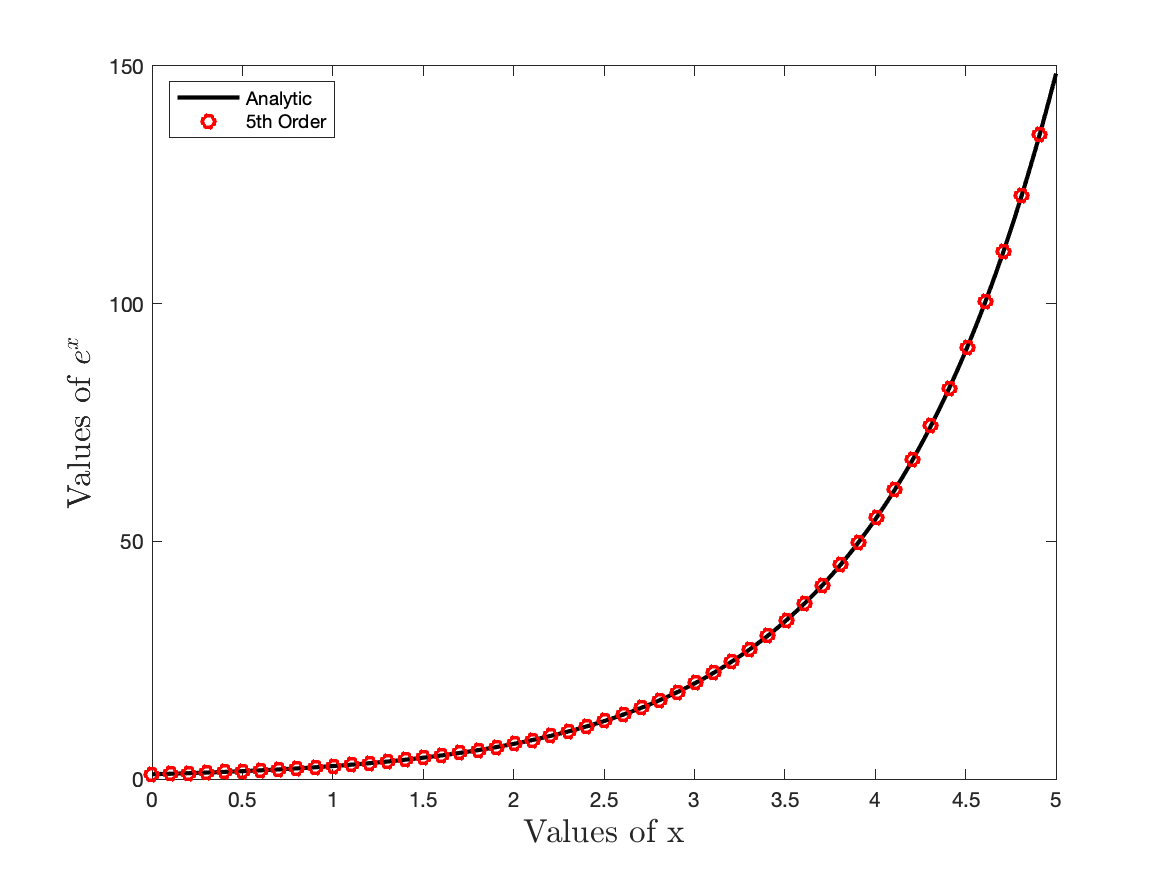
\includegraphics[width=1.1\columnwidth]{figs/1stDer.png}
		\label{fig:1stDer} 
		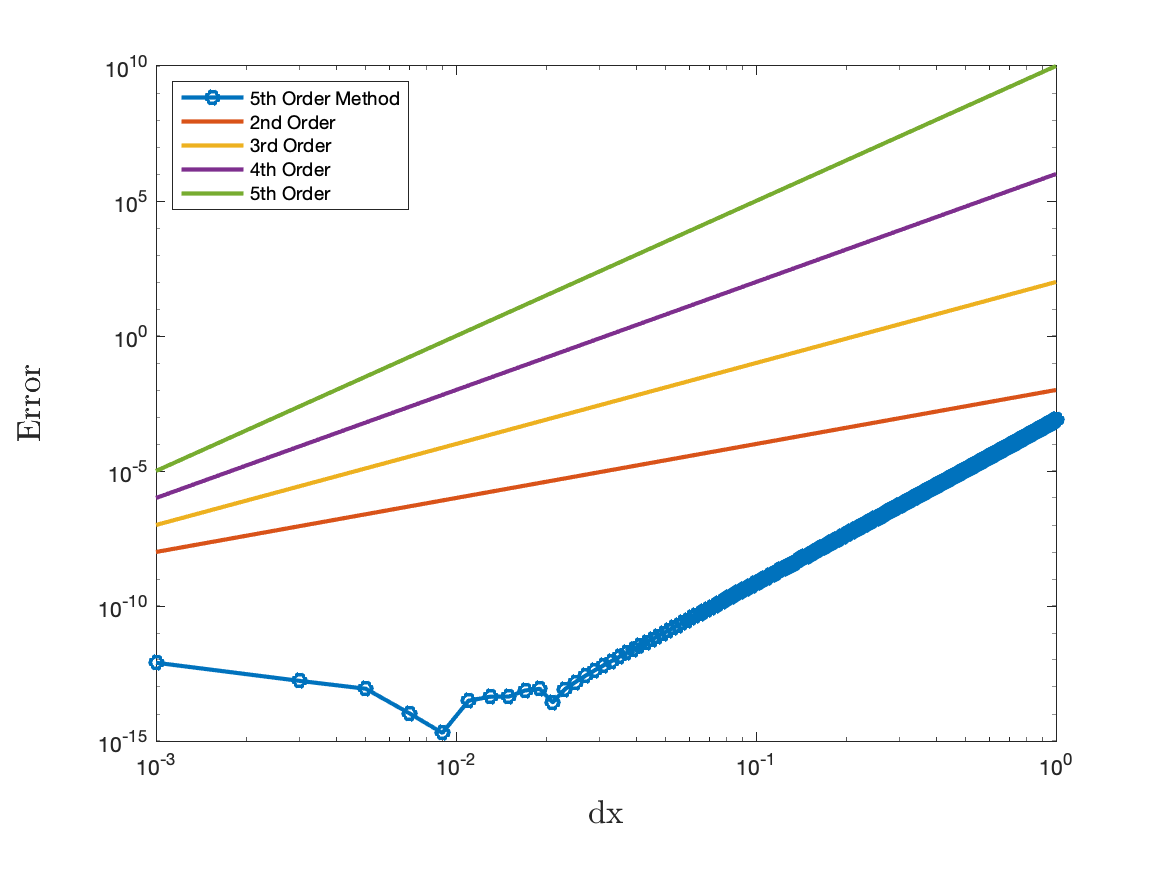
\includegraphics[width=1.1\columnwidth]{figs/1stErr.png}
		\label{fig:1stDer} 
	\end{multicols}
	\caption{First derivative results.\hl{FIGURE OUT WHAT TO DO ABOUT THIS}}
\end{figure}

\begin{figure}
	\begin{multicols}{2}
		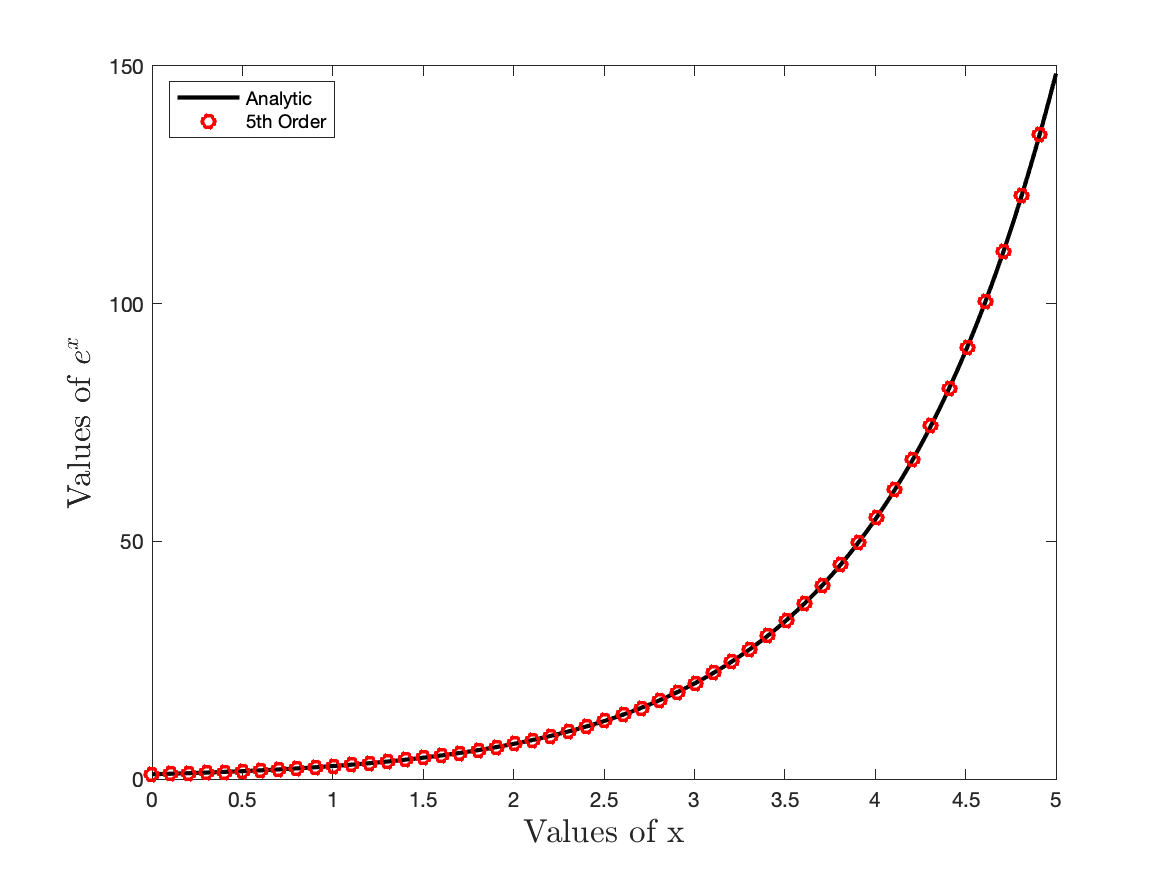
\includegraphics[width=1.1\columnwidth]{figs/2ndDer.png}
		\label{fig:2ndDer} 
		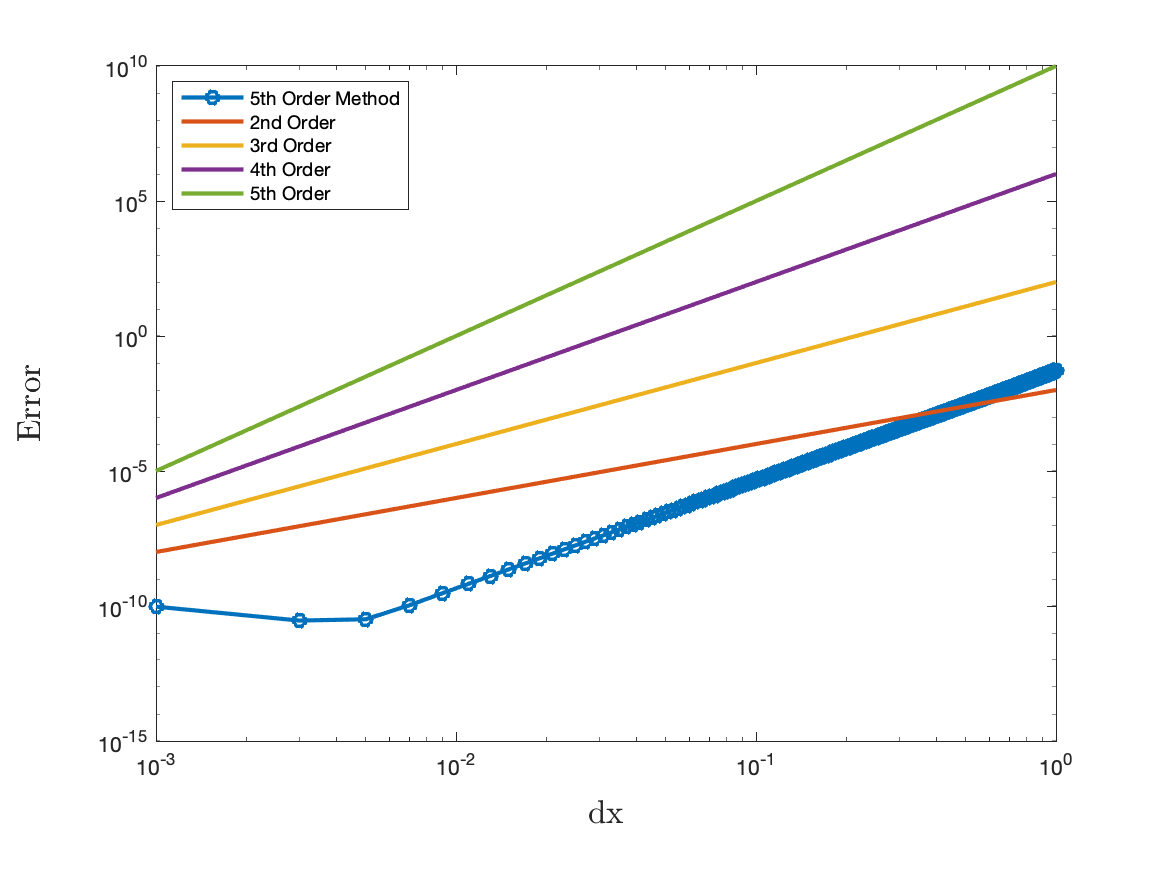
\includegraphics[width=1.1\columnwidth]{figs/2ndErr.png}
		\label{fig:2ndErr} 
	\end{multicols}	
		\caption{Second derivative results.\hl{FIGURE OUT WHAT TO DO ABOUT THIS}}
\end{figure}


 The simplest test case for testing a curvature scheme is to compute the curvature of an exact VOF field. The curvature of a circle for example, is exactly equal to the reciprocal of the radius as seen in Figure~\ref{fig:curv}. We establish a simple case where a circle is given a radius of 0.2. Figure~\ref{fig:5thcurv} shows the resulting curvature field for this geometry. Results indicating that the method is performing as anticipated and accuracy increases with mesh refinement. With the successful implementation and initial calculation, the method was again tested using the oscillating droplet test case. Figure~\ref{fig:5thKE} shows the total kinetic energy with time throughout the course of the simulation. Here, instead of the dissipation of kinetic energy we see behavior similar to that of the standard height function method. The scheme is stable initially and then kinetic energy grows uncontrollably until eventual simulation failure.
\begin{figure}[htbp]
	\centering
	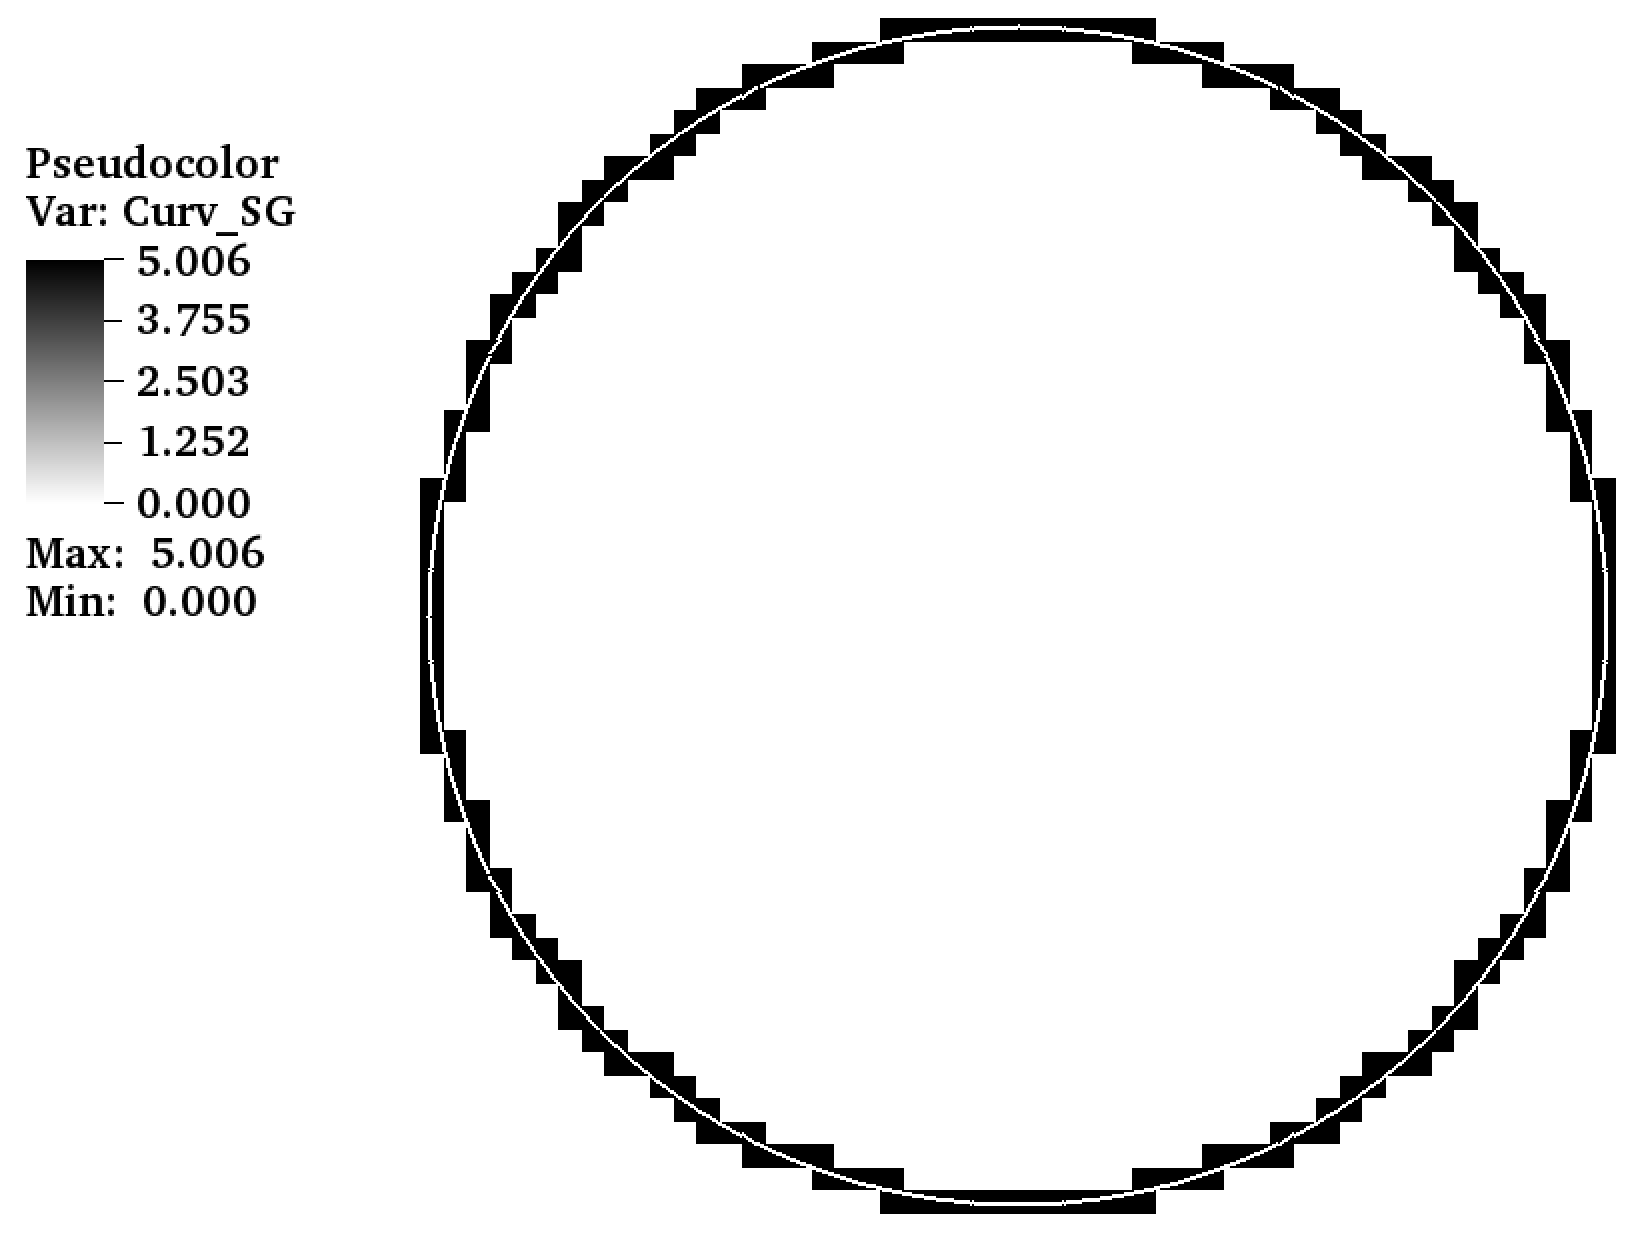
\includegraphics[width=0.5\textwidth]{figs/curvCalc.png}
	\caption{$5^{th}$ order scheme.\hl{THIS IS NOT THE CORRECT FIGURE}}
	\label{fig:5thcurv} 
\end{figure} 

\begin{figure}[h]
	\centering
	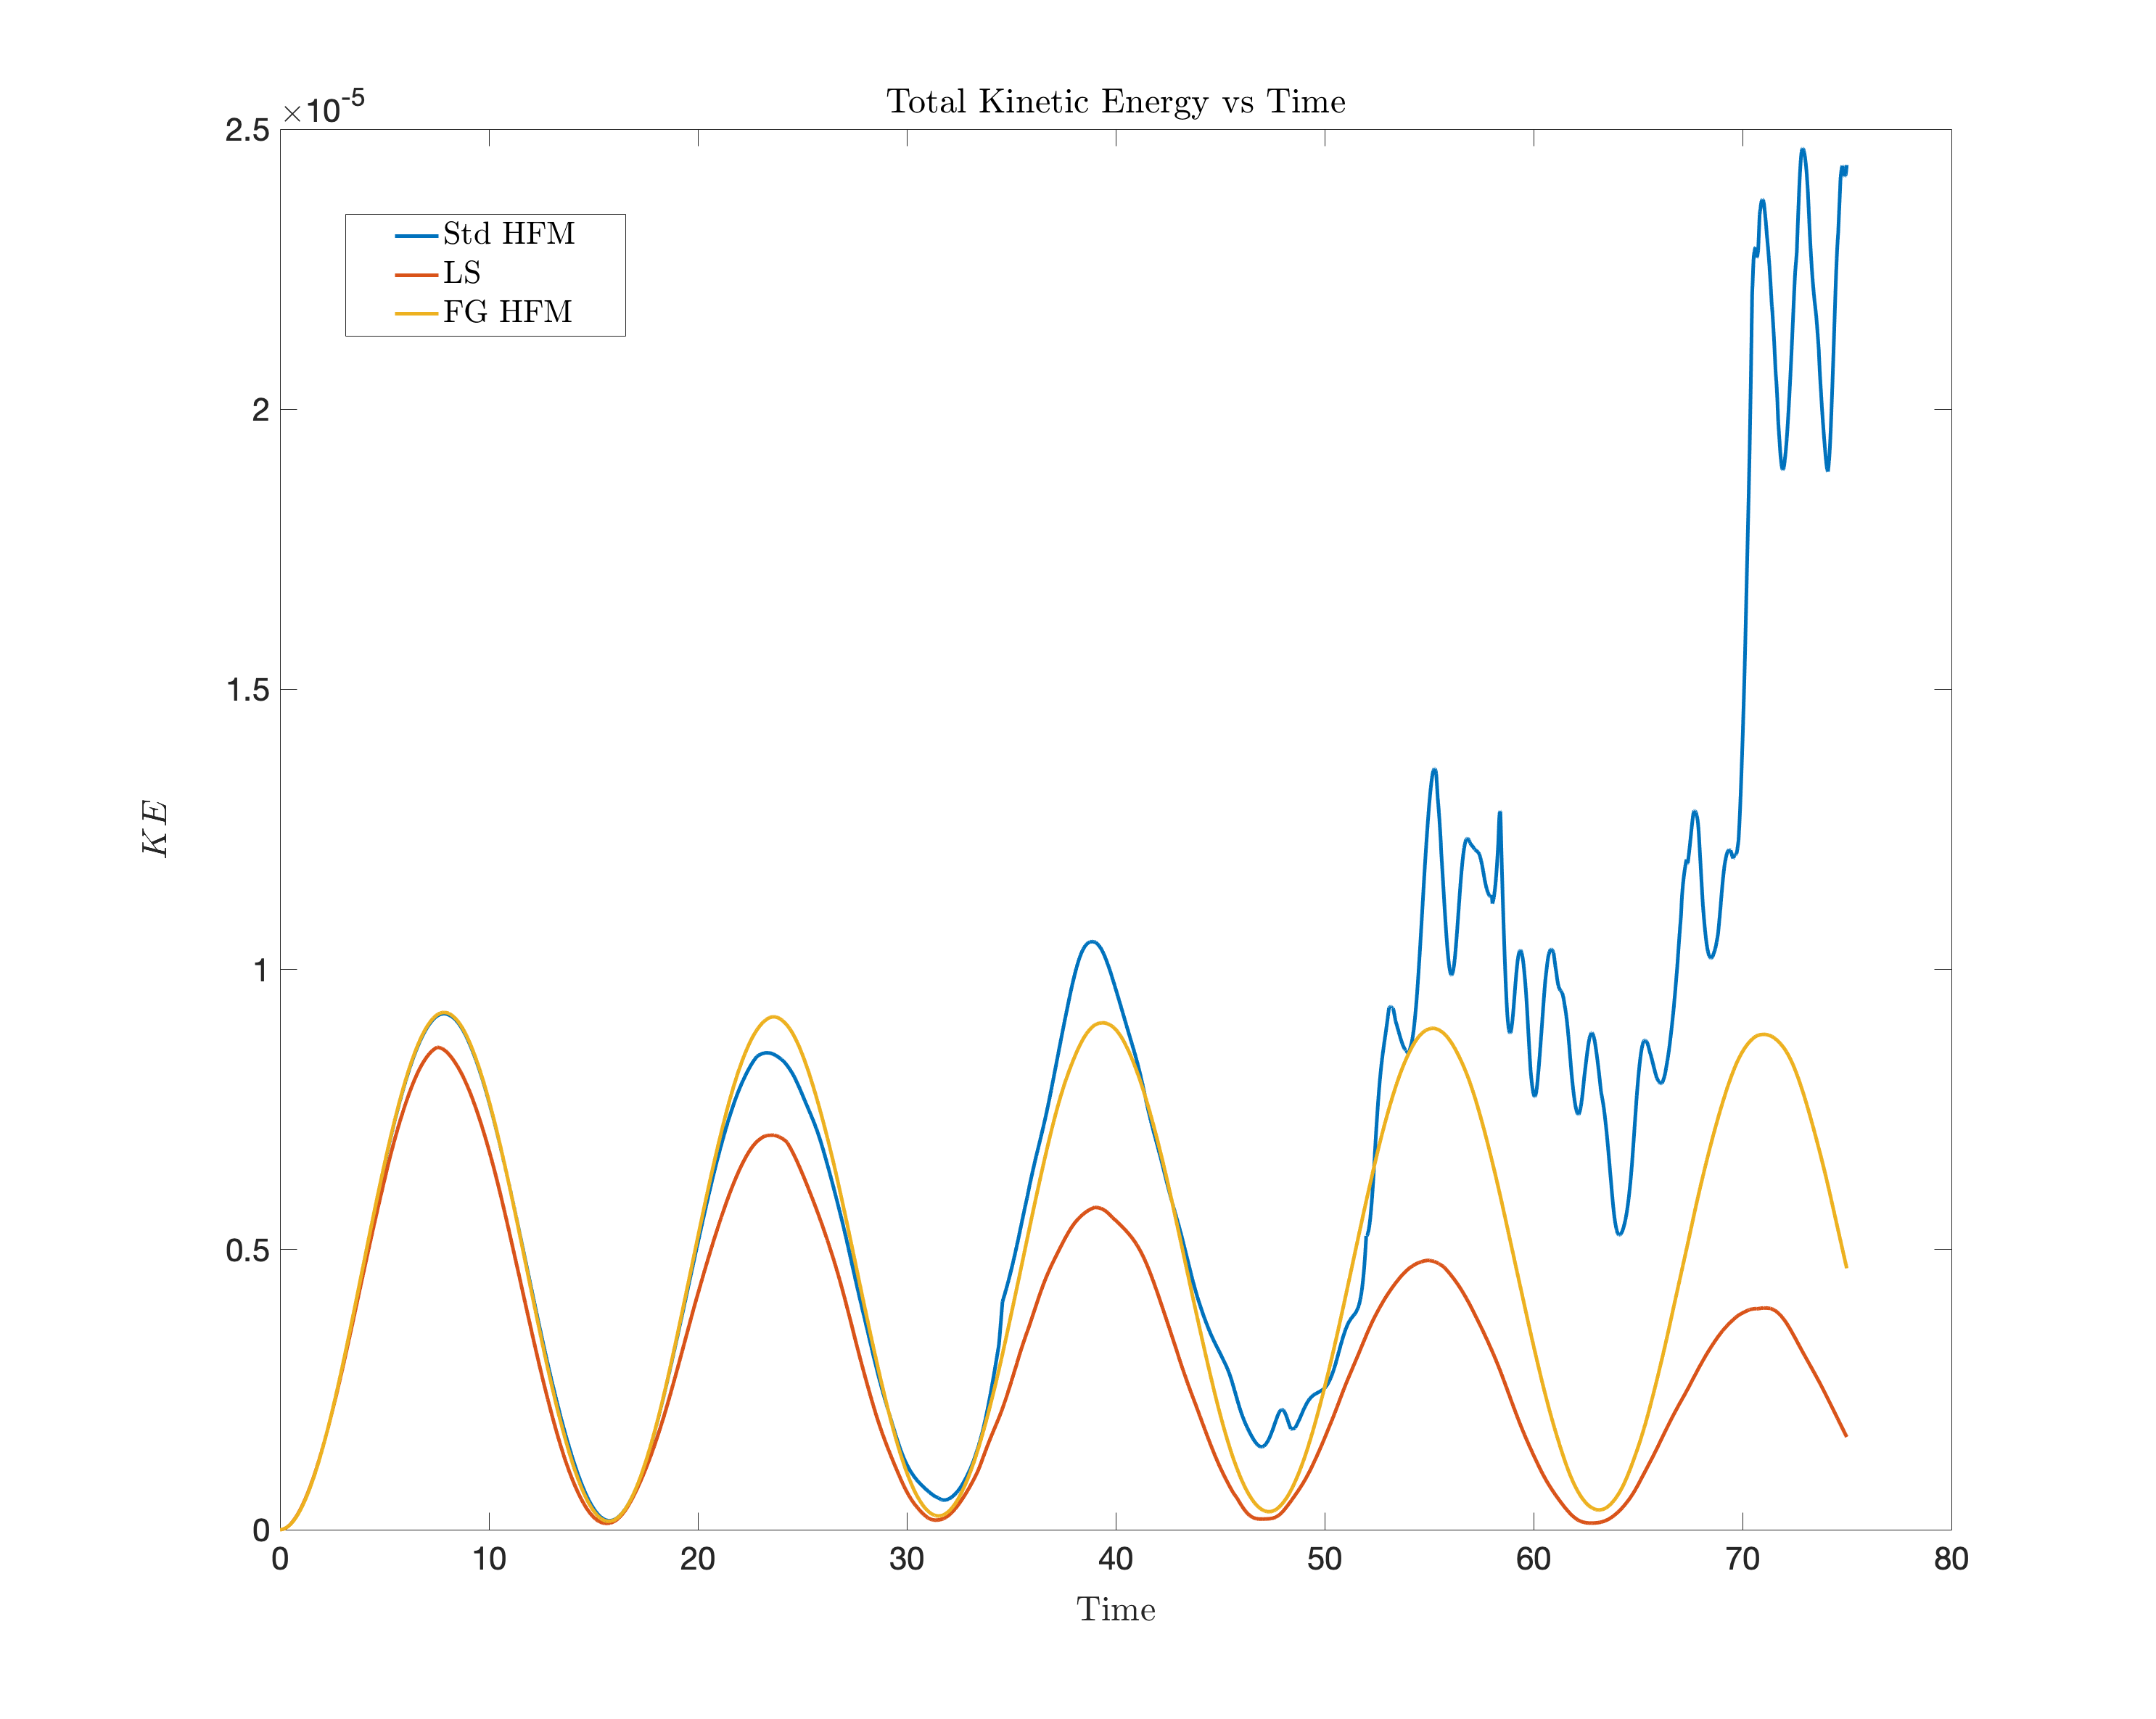
\includegraphics[width=0.5\textwidth]{figs/KEvT}
	\caption{Kinetic Energy with Time \hl{THIS IS NOT THE CORRECT FIGURE}}
	\label{fig:5thKE}
\end{figure}

\subsection{Importance of Scale}
 Fifth order polynomials as used here, can have large oscillations in the curvature calculation leading to the observed errors in figure \ref{fig:5thKE}.This error is likely due to the scheme being influenced by areas of both highly positive and highly negative curvature within the fit. In a 2018 article, Owkes et al.~found that the scale with which curvature is computed on heavily influences the growth of interface perturbations~\cite{Owkes2018}.This article also suggested that at certain scales, a second order method was more agreeable with accurate interface dynamics than a fourth order method on the same scale~\cite{Owkes2018}. With this, we considered the possibility that a fifth order function on the fine grid scale may be over-fitting the points and reconstructing an interface with more perturbations than actually exist, essentially exacerbating our problem as opposed to alleviating it. Figure~\ref{fig:draw} shows an example of what this may look like. 

\begin{figure}[htbp]
	\centering
	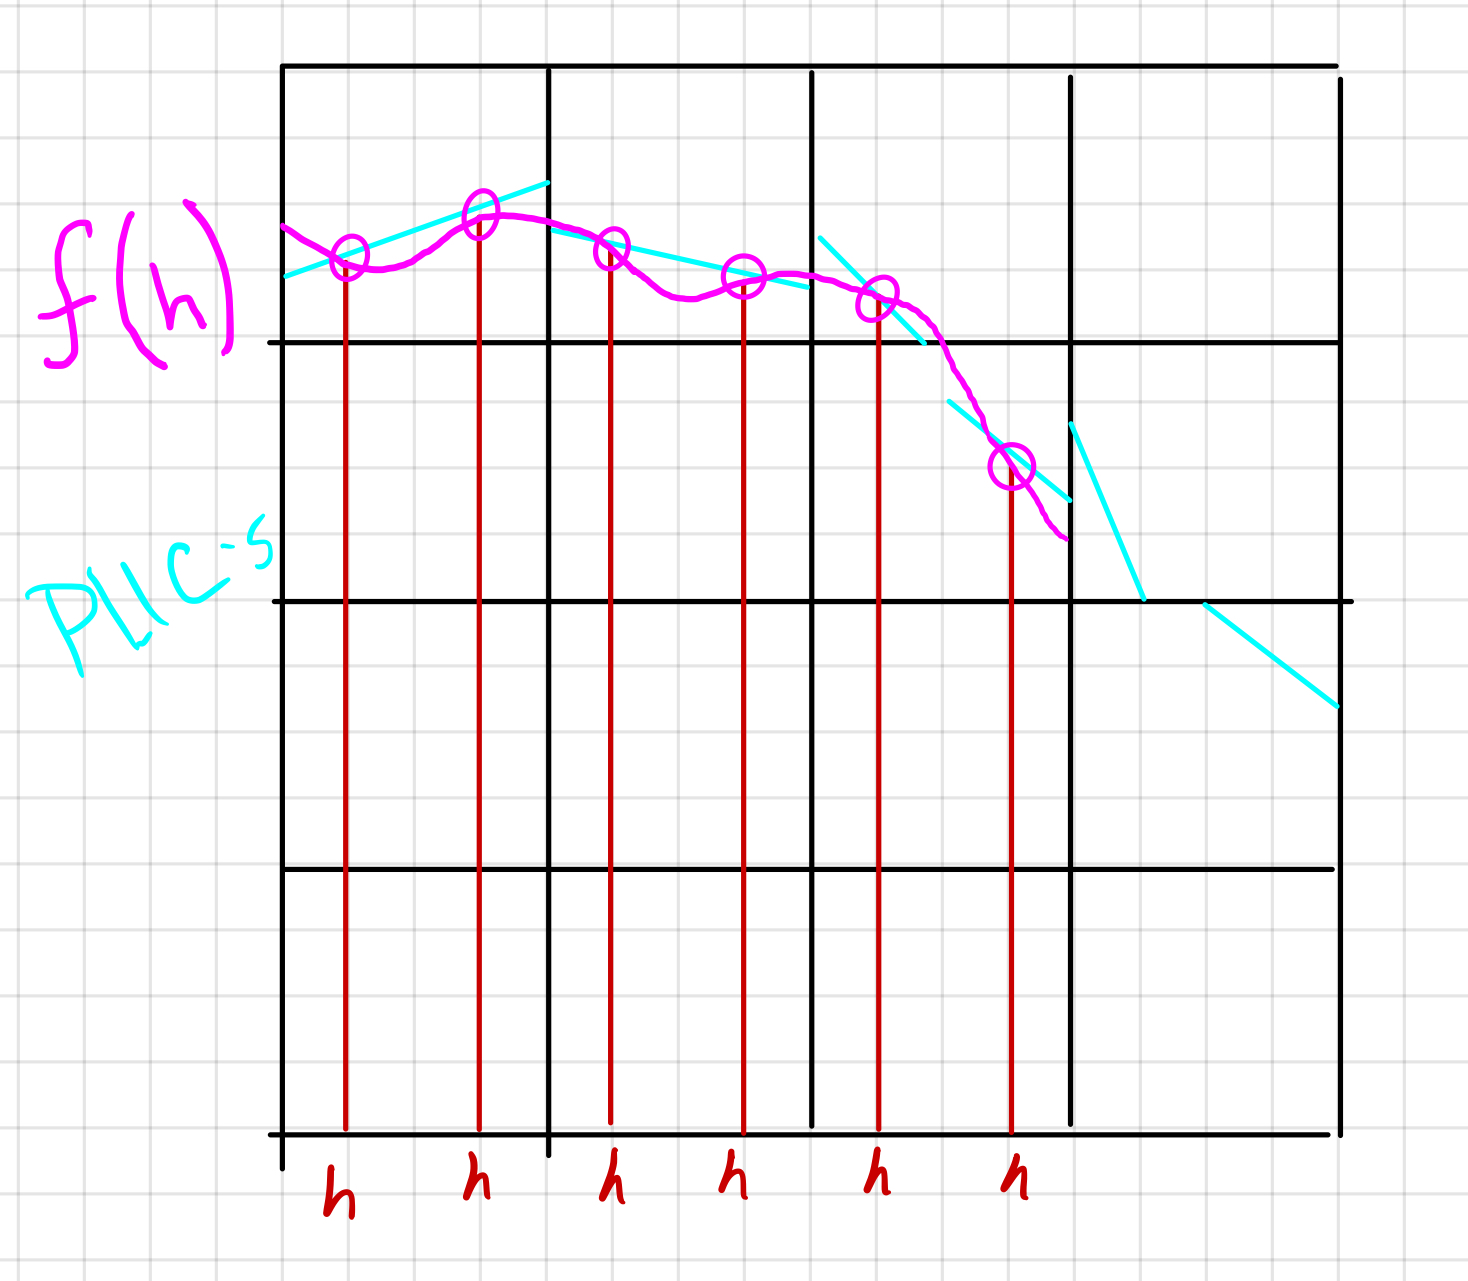
\includegraphics[width=0.5\textwidth]{figs/draw}
	\caption{\hl{Draw something that gives the same message}}
	\label{fig:draw}
\end{figure}

\subsection{Second Order Fine Grid Height Function Method}
Because the error order of a method comes second to accurately representing physical dynamics, we decided to use the same stencil but pass a 2nd order polynomial through the points. The general idea is represented in Figure~\ref{fig:2ndhts}. Calculating a 2nd order method was done using the same general finite difference technique as described previously but to 2nd order accuracy. The same symmetry assumption as made previously lead to undetermined operators that could be used as a tuning parameters. The aim of this method would be to use the same fine grid information to inform the coarse model but to smear the function to reduce unwanted perturbations. Again with mesh refinement, calculation of an exact curvature field produced encouraging results as seen in Figure~\ref{fig:2ndCurv.png}.   Parameterization of the free variables allows for an optimized solution which produces more favorable results than the fifth order method as seen in Figure~\ref{fig:2ndKE}. However, the method still allows for the uncontrolled growth of fine grid fluctuations which results in simulation failure. 

\begin{figure}[htbp]
	\centering
	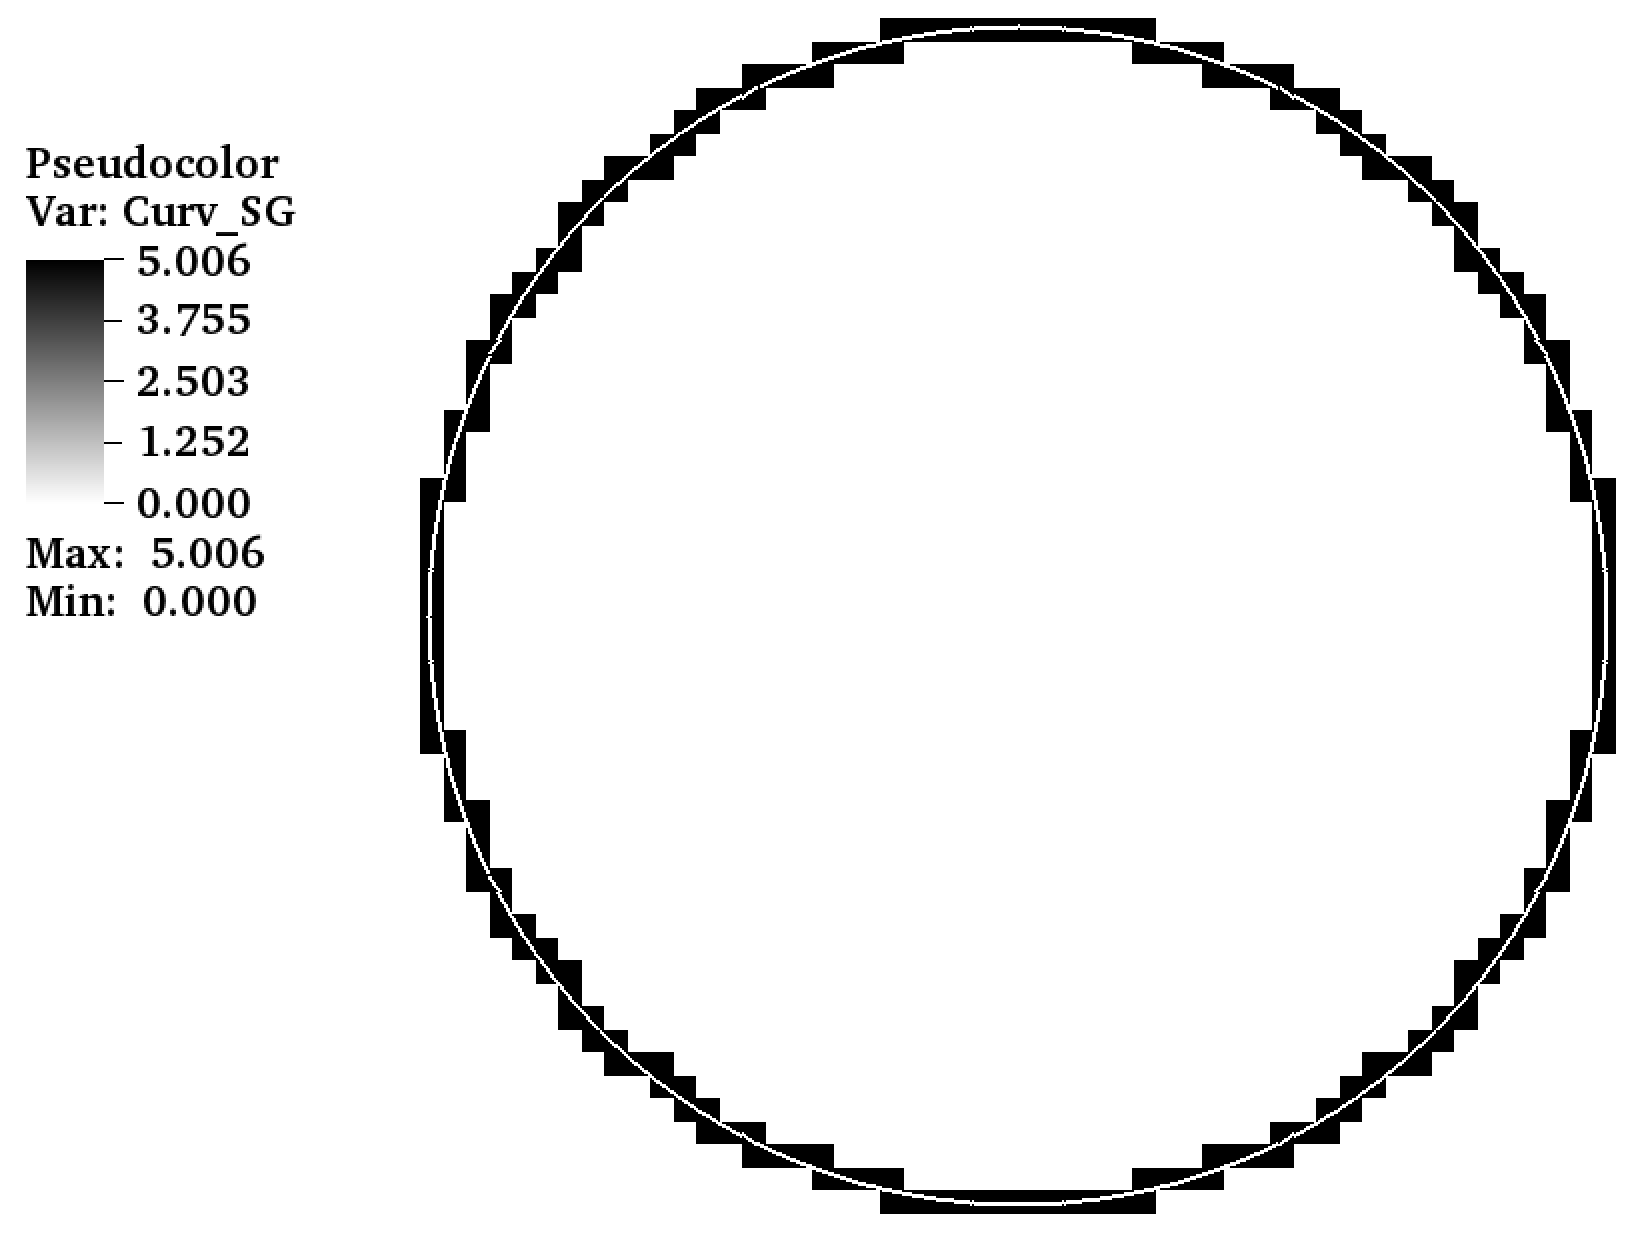
\includegraphics[width=0.5\textwidth]{figs/curvCalc.png}
	\caption{$2^{nd}$ order scheme.\hl{THIS IS NOT THE CORRECT FIGURE}}
	\label{fig:2ndCurv} 
\end{figure} 

\begin{figure}[htbp]
	\centering
	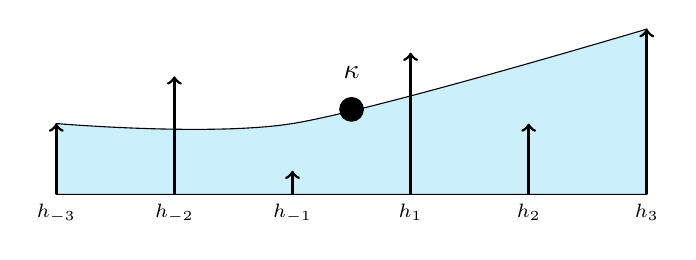
\begin{tikzpicture}[scale=3.0]
	\draw [black, fill=cyan!20] plot [smooth ] coordinates {(0.25,0.3)(1.25,0.3)(2.75,0.7)} -- (2.75,0) -- (0.25,0) -- cycle;
	\draw [fill] (1.5,0.36) circle [radius=0.05];
	\node [above ] at (1.5,0.45) {$\kappa$};
	\draw [arrows=->,line width=1.0] (0.25,0) -- (0.25,0.3);\node [below] at (0.25,0) {\scriptsize $h_{-3}$};
	\draw [arrows=->,line width=1.0] (0.75,0) -- (0.75,0.5);\node [below] at (0.75,0) {\scriptsize $h_{-2}$};
	\draw [arrows=->,line width=1.0] (1.25,0) -- (1.25,0.1);\node [below] at (1.25,0) {\scriptsize $h_{-1}$};
	\draw [arrows=->,line width=1.0] (1.75,0) -- (1.75,0.6);\node [below] at (1.75,0) {\scriptsize $h_{1}$};
	\draw [arrows=->,line width=1.0] (2.25,0) -- (2.25,0.3);\node [below] at (2.25,0) {\scriptsize $h_{2}$};
	\draw [arrows=->,line width=1.0] (2.75,0) -- (2.75,0.7);\node [below] at (2.75,0) {\scriptsize $h_{3}$};	
	\end{tikzpicture}
	\caption{$2^{nd}$ Order Fit}
	\label{fig:2ndhts}
\end{figure}

\begin{figure}[h]
	\centering
	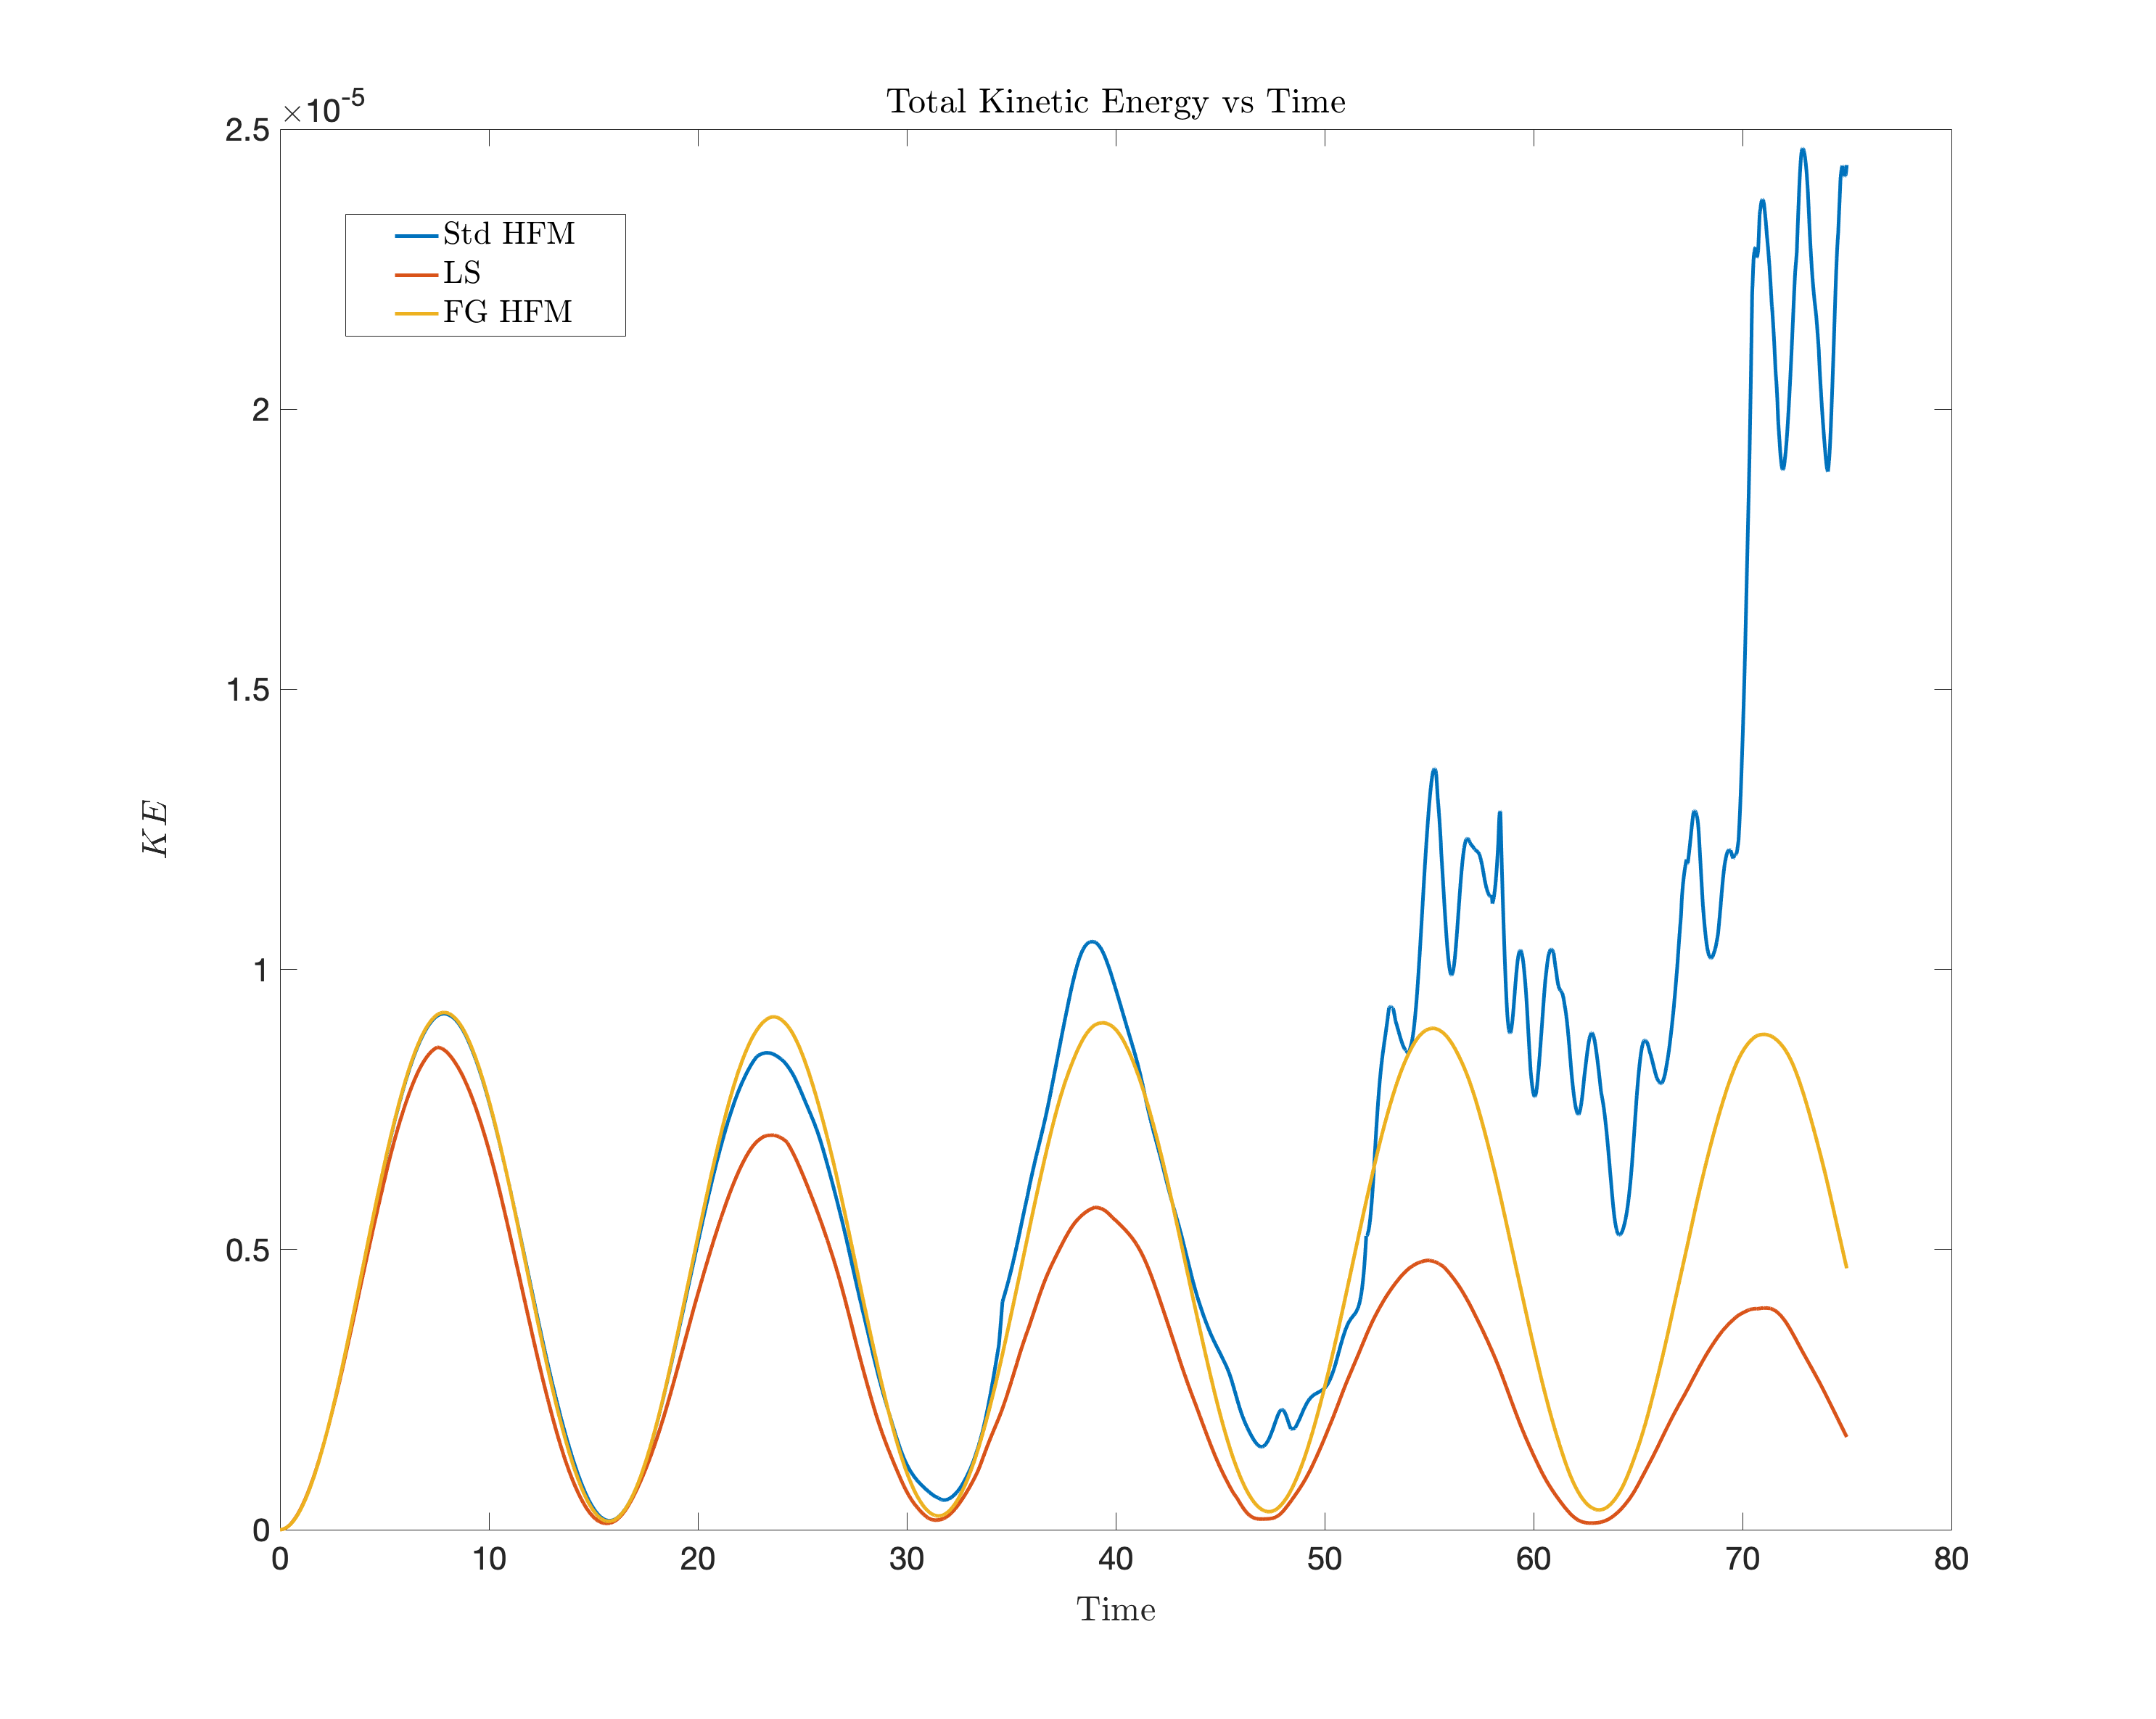
\includegraphics[width=0.5\textwidth]{figs/KEvT}
	\caption{Kinetic Energy with Time \hl{THIS IS NOT THE CORRECT FIGURE}}
	\label{fig:2ndKE}
\end{figure}


\subsection{Gaussian Filtering Second Order Method}

In the 5th order method, curvature is evaluated at the center of the stencil. However, a more reasonable curvature can be obtained by computing an average curvature over the stencil. This is done by filtering equation \ref{eqn:poly} with a Gaussian distribution as in equation \ref{eqn:filt}. This smooths the polynomial and allows for a more realistic estimation of the curvature. Averaging is achieved using a convolution with a weighting kernel. Transition to $\zeta$ space simplifies this scheme and is defined as $\zeta = \frac{2}{\Delta x}(x-x_i)$. This scheme requires only one floating variable ($\sigma$) as seen in equation \ref{eqn:G}. Varying this parameter modifies the scale and filtering kernel of the scheme, allowing optimal operating parameters to be determined. Here, scale refers to the size of the computational stencil with which the curvature is computed as previously described by Owkes et al. \cite{Owkes2018}. As seen in figure \ref{fig:GPlot}, the result is better than previous iterations and is significantly more accurate than the standard height function method. However, this model also provides undesirable results at later time steps.     

\vspace{-0.2in}
\begin{equation}
\kappa = \int_{-3}^{3} G(\zeta) \kappa(\zeta) d\zeta
\label{eqn:filt}
\end{equation} 
\begin{equation}
G(\zeta) = \frac{1}{\sqrt{2 \pi \sigma^2}}e^\frac{- \zeta^2}{2\sigma^2}
\label{eqn:G}
\end{equation} 

\begin{figure}[htbp]
	\centering
	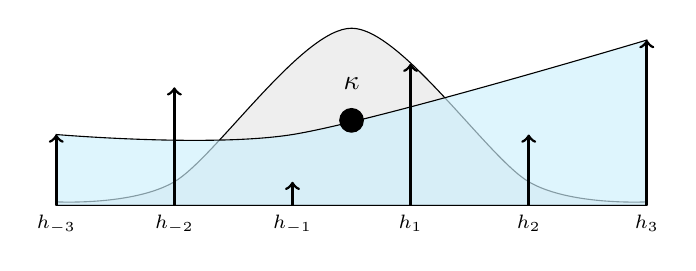
\begin{tikzpicture}[scale=3.0]
	\begin{scope}[fill opacity=0.65]
	\draw [black, fill=gray!20] plot [smooth ] coordinates {(0.25,0.015)(0.75,0.1)(1.50,0.75)(2.25,0.1)(2.75,0.015)} -- (2.75,0) -- (0.25,0) -- cycle;
	
	\draw [black, fill=cyan!20] plot [smooth ] coordinates {(0.25,0.3)(1.25,0.3)(2.75,0.7)} -- (2.75,0) -- (0.25,0) -- cycle;
	\end{scope}
	\draw [fill] (1.5,0.36) circle [radius=0.05];
	\node [above ] at (1.5,0.45) {$\kappa$};
	\draw [arrows=->,line width=1.0] (0.25,0) -- (0.25,0.3);\node [below] at (0.25,0) {\scriptsize $h_{-3}$};
	\draw [arrows=->,line width=1.0] (0.75,0) -- (0.75,0.5);\node [below] at (0.75,0) {\scriptsize $h_{-2}$};
	\draw [arrows=->,line width=1.0] (1.25,0) -- (1.25,0.1);\node [below] at (1.25,0) {\scriptsize $h_{-1}$};
	\draw [arrows=->,line width=1.0] (1.75,0) -- (1.75,0.6);\node [below] at (1.75,0) {\scriptsize $h_{1}$};
	\draw [arrows=->,line width=1.0] (2.25,0) -- (2.25,0.3);\node [below] at (2.25,0) {\scriptsize $h_{2}$};
	\draw [arrows=->,line width=1.0] (2.75,0) -- (2.75,0.7);\node [below] at (2.75,0) {\scriptsize $h_{3}$};
	\end{tikzpicture}
	%						\caption{Gaussian Fit}
	%						\label{fig:Ghts} 
\end{figure}

\subsection{Implementation of Fine Grid Velocities}
\hl{this is pulled from ILASS paper, consider rewriting this...talk more about how the implication is now that we are dealing with differences in curvature so we have tried several ways of representing coarse grid curv (avg of fg, weighted avg, std hfm) as well as adding another pressure eqn }

As previously mentioned, the inclusion of a fine grid allows for the existence of fine grid interfacial perturbations. While the fine grid height function method does provide a more rigorous representation of curvature, it does not reduce or remove the interfacial perturbations which exist on the fine mesh. To reduce the influence of these perturbations a fine grid velocity is implemented based on the work of Herrmann~\cite{Herrmann2013}. 

A spring-damper analogy is used to approximate interface motion, \ie,
\begin{equation}
\frac{\partial \bm{u}_{\text{fg}}}{\partial t} +
(\bar{\bm{u}}+\bm{u}_{\text{fg}}) \cdot \nabla \bm{u}_{\text{fg}} = 
c_{\sigma}\frac{\sigma}{\rho}\bar{\kappa}(\kappa_{\text{fg}}-\bar{\kappa})- 
c_{\mu}\frac{\mu}{\rho L^2}\bm{u}_{\text{fg}}\nonumber
\label{HermEq}
\end{equation}

where, $\bar{\bm{u}}$ is the resolved velocity,
$\bm{u}_{\text{fg}}$ is the fine grid velocity,
$\sigma$ is the surface tension coefficient,
$\rho$ is density, 
$\bar{\kappa}$ is the resolved curvature,
$\kappa_{\text{fg}}$ is the fine grid curvature,
$\mu$ is the dynamic viscosity,
$L$ is a modeling length scale and
$C_\sigma$ and
$C_\mu$ are surface tension and viscous scaling coefficients, respectively~\cite{Herrmann2013}. 
The left side of the equation includes a velocity time rate of change as well as a convective term, while the right side includes the surface tension term which acts as a spring force and the viscous term which is analogous to a damping force. By this analogy, system behavior can be moderated by scaling the value on the surface tension or viscous coefficients. Close inspection of Eq.~\ref{HermEq} reveals that the equation is not well-poised when the coarse-grid curvature, $\bar{\kappa}$, is zero as the entire spring force goes to zero even if fine-grid interface perturbations exist.  An alternative is to base the source term on the difference between coarse and fine-grid curvatures and add a delta function that restricts the source term to only be non-zero at the interface.  The approximation of the Dirac delta function is calculated as the absolute difference in liquid volume fractions between cells divided by the mesh size. Additionally, a pressure term is added to ensure fine grid velocity remains divergence free, further enforcing momentum conservation. With these modifications, the proposed equation to create the fine-grid velocity can be written as

\begin{equation}
\frac{\partial \bm{u}_{\text{fg}}}{\partial t} +
(\bar{\bm{u}}+\bm{u}_{\text{fg}}) \cdot \nabla \bm{u}_{\text{fg}} = 
c_{\sigma}\frac{\sigma}{\rho}\delta(\kappa_{\text{fg}}-\bar{\kappa})- 
c_{\mu}\frac{\mu}{\rho L^2}\bm{u}_{\text{fg}} -
\nabla P_{\text{fg}}\nonumber
\label{MyEq}
\end{equation}
along with the continuity equation
\begin{equation}
\nabla\cdot\bm{u}_\text{fg}=0.
\end{equation}

\subsection*{Correction Incorporation} 
\hl{talk more about fluxes and streaktubes... have room to go into detail}

Away from the phase interface, NGA uses arbitrarily high-order finite difference operators that conservatively transport mass, momentum, and any other scalars~\cite{NGA2}.  These operators are well suited for simulations of turbulent flows.  Near the phase interface the finite difference operators are inappropriate due to discontinuities.  Alternatively, an unsplit geometric semi-Lagrangian VoF method is leveraged~\cite{Owkes2017,Owkes2014}.

Adding the fine-grid velocity correction is done by modifying the additional flux due to the fine-grid velocities.  For the finite difference scheme this entails adding the fine-grid velocities associated with a cell face onto the convection velocity at that face.  The semi-Lagrangian fluxes are modified as described below.

In the semi-Lagrangian scheme, a streaktube is constructed that contains the region of the domain that moves through a computational cell face during the timestep~\cite{Owkes2017}.  The streaktube is represented with a collection of tetrahedra and computational geometry is used to compute the flux of liquid, mass, momentum, and any scalars~\cite{Owkes2017}. Including the fine-grid velocity requires modifying the streaktubes and in this work two additional tetrahedra are added to each subface such that the volume of the additional tetrahedra is equal to $V_\text{tets}=\Delta t \mathcal{A}_\text{face} \bm{u}_\text{fg}\cdot\bm{n}$. This addition provides an explicit numerical representation of the fine grid velocity correction and maintains conservation laws. 



















